\documentclass{beamer}
\title{Snails}
\author{Craig \and Milan \and Jack}
\date{20th June}
\usetheme{AnnArbor}
\usecolortheme{dolphin}
\setbeamertemplate{navigation symbols}{} 

\AtBeginSection
{
  \begin{frame}{Outline}
    \tableofcontents[currentsection]
  \end{frame}
}

\begin{document}

\begin{frame}
  \titlepage
\end{frame}

\section{Introduction}

\begin{frame}{Introduction}
  We did a game about snails and we think it is pretty cool and you guys should probably check it out or something. \\
  \vspace{\baselineskip}
  I mean, no pressure, but it is pretty awesome.
\end{frame}


\section{The Game}
\subsection{Aesthetics}

\begin{frame}{Art and Animation}
\end{frame}

\begin{frame}{User Interface}
\end{frame}

\subsection{Game Background}

\begin{frame}{Background Story}
  So, right, basically, what you have, right, is these ghosts and stuff. \\
  \vspace{\baselineskip}
  Also, there's all these, like, snails and stuff. \\
  \vspace{\baselineskip}
  They are not friends. \\
  \vspace{\baselineskip}
  :(
\end{frame}

\begin{frame}{Game Rules}
  \begin{itemize}
    \item Rule 1
    \item Rule 2
    \item We don't need more than 2 rules
  \end{itemize}
\end{frame}


\section{Group Management}

\begin{frame}{Git}
\end{frame}

\begin{frame}{Pivotal Tracker}
  Clear structure.\\
  \begin{figure}[hb]
    \centering
    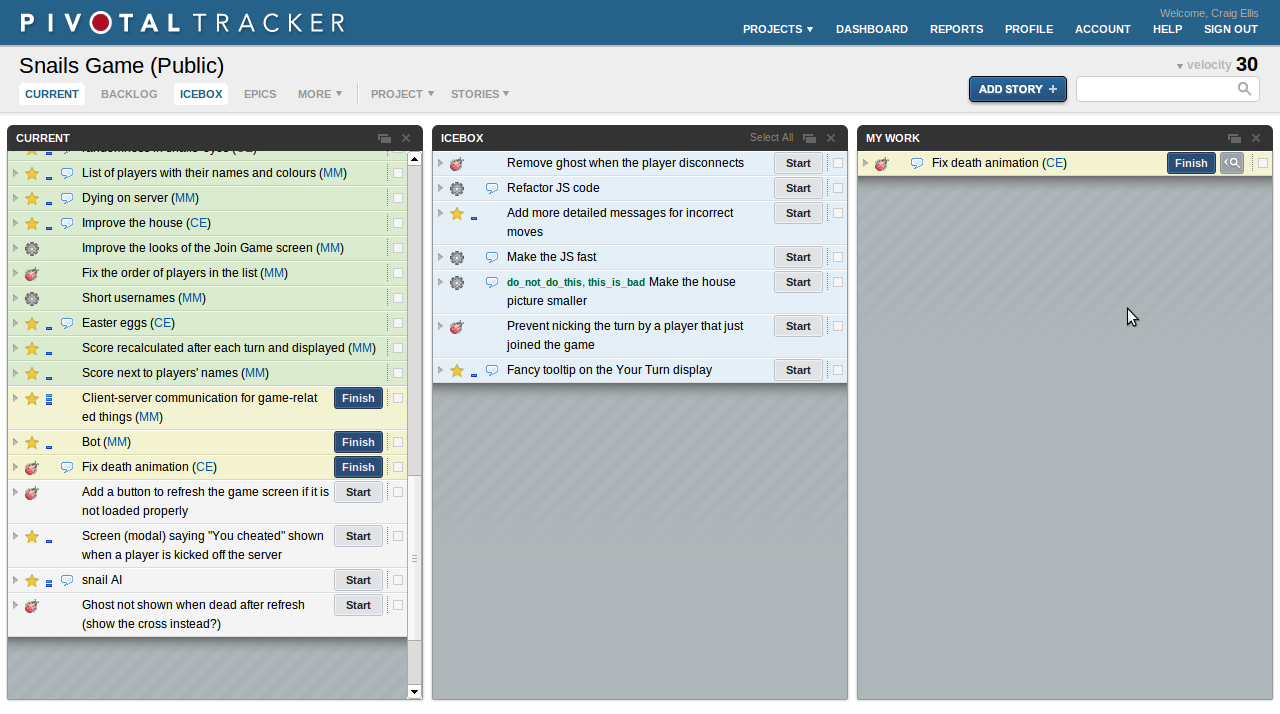
\includegraphics[scale=0.2]{pivotal.png}
    \caption{Look at the nice tracker}
  \end{figure}
\end{frame}


\section{Implementation Languages}
\subsection{Client}

\begin{frame}{Javascript}
  [insert map of components and interactions.]
  \begin{itemize}
    \item Suitable for purpose
    \item It's nice
    \item We like it
    \item Also paper.js
  \end{itemize}
\end{frame}

\begin{frame}{HTML5}
  [insert map of components and interactions.]
  \begin{itemize}
    \item Suitable for purpose
    \item It's nice
    \item We like it
  \end{itemize}
\end{frame}

\subsection{Server}

\begin{frame}{Django}
  [insert map of components and interactions.]
  \begin{itemize}
    \item Suitable for purpose
    \item It's nice
    \item We like it
  \end{itemize}
\end{frame}

\begin{frame}{Heroku}
  [insert map of components and interactions.]
  \begin{itemize}
    \item Suitable for purpose
    \item It's nice
    \item We like it
  \end{itemize}
\end{frame}


\section{Conclusion}

\begin{frame}{Conclusion}
  [insert reflection on project outcomes.]
\end{frame}

\end{document}
